\documentclass[a4paper,twocolumn]{article}
\usepackage[utf8]{inputenc}
\usepackage[T2A]{fontenc}
\usepackage{fancyhdr}
\usepackage{csquotes}
\usepackage{hyperref}
\usepackage{graphicx}
\usepackage{wrapfig}
\usepackage{sverb}
\usepackage{lastpage}
\usepackage{listings}
\usepackage{enumitem}
\usepackage{amssymb}
\usepackage{amsmath}
\usepackage{lscape}

% \usepackage[russian]{babel}

% \usepackage{pdflscape}



\usepackage[left=1cm, right=1cm, top=2cm, bottom=1.5cm, landscape]{geometry}


\lstset{
  basicstyle=\ttfamily,
  columns=fixed,
  fontadjust=true,
  basewidth=0.5em
}



\hypersetup{
    colorlinks=true,       % Enable colored links
    linkcolor=blue,        % Color for internal links (e.g., sections, equations)
    filecolor=magenta,     % Color for linked files
    urlcolor=cyan,         % Color for external hyperlinks
    pdftitle={Meow}, % PDF metadata title
}

\pagestyle{fancy}
\lhead{HSE <<idk>> (MacNeil, Martynov, Piskarev)}
\rhead{\thepage\ of \getpagerefnumber{LastPage}}
% \pagenumbering{gobble}


\begin{document}



\small
\tableofcontents


\tiny
\footnotesize
\scriptsize

% \section{}

\subsubsection{sum kth powers}
\lstinputlisting{src/sum_kth_powers.txt}
% 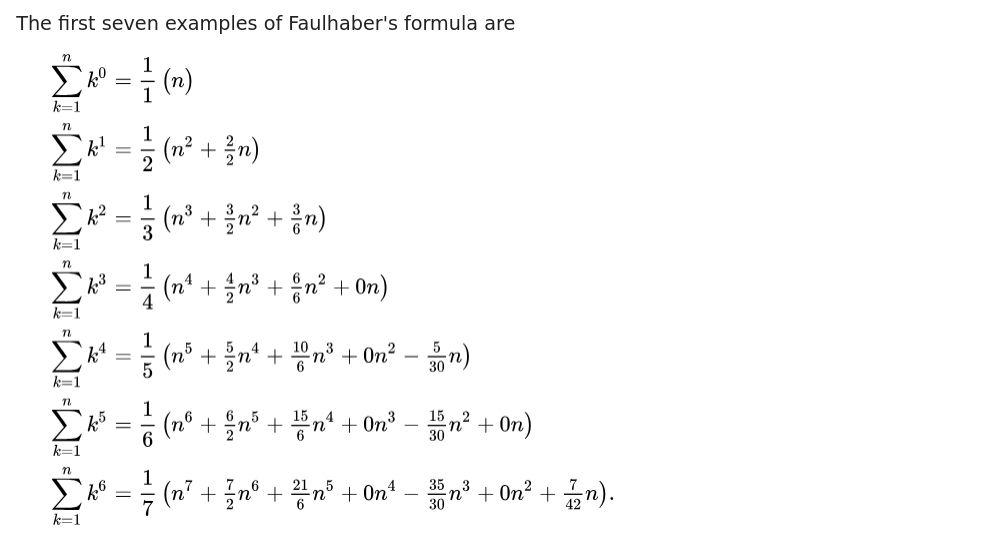
\includegraphics[width=0.42\textwidth]{src/sum_kth_powers.png}
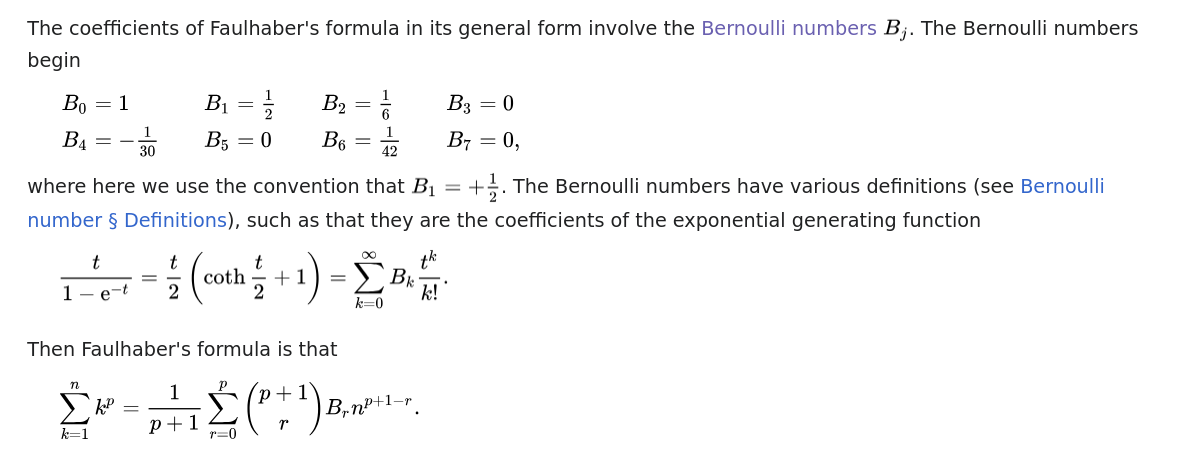
\includegraphics[width=0.42\textwidth]{src/sum_kth_powers_2.png}
% 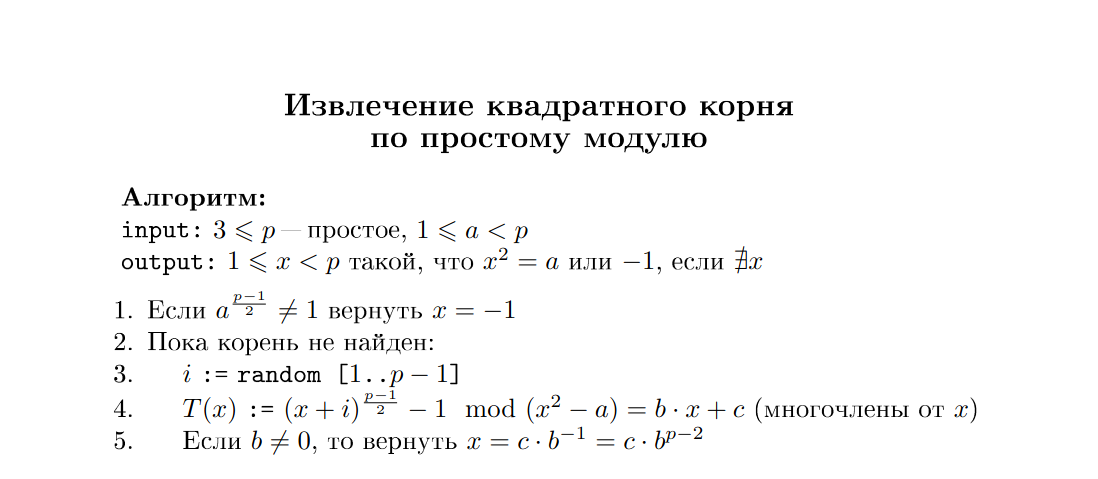
\includegraphics[width=0.42\textwidth]{src/prime_sqrt.png}

\subsubsection{hcn}
\lstinputlisting{src/hcn.txt}

\subsubsection{******** general matching}
\lstinputlisting{src_compressed/blossom.cpp}


\subsubsection{svg}
\lstinputlisting{src_compressed/svg.cpp}

\subsubsection{floor sum + mod linear}
\lstinputlisting{src_compressed/fisting_mod.cpp}

% \subsubsection{ntt}
% \lstinputlisting{src_compressed/ntt_short.cpp}

% \subsubsection{simd binsearch int32}
% \lstinputlisting{src_compressed/simd_binsearch.cpp}

\subsubsection{primality test + Rho factorization}
\lstinputlisting{src_compressed/factorize.cpp}

% \subsubsection{Flow}
% \lstinputlisting{src_compressed/flow.cpp}


% \subsubsection{simd merge + compress}
% \lstinputlisting{src_compressed/simd_merge.cpp}

\subsubsection{tree bitset}
\lstinputlisting{src_compressed/tree_bitset.cpp}

\subsubsection{link cut}
\lstinputlisting{src_compressed/link_cut.hpp}

\subsubsection{simplex}
\lstinputlisting{src_compressed/simplex.hpp}

\subsubsection{suffix array}
\lstinputlisting{src_compressed/SA_IS.hpp}


\subsubsection{dom tree}
\lstinputlisting{src_compressed/dom.cpp}

\subsubsection{poly}
\lstinputlisting{src_compressed/poly.hpp}

\subsubsection{multipoint}
\lstinputlisting{src_compressed/multi_eval.hpp}


\subsubsection{******** ntt}
\lstinputlisting{src_compressed/ntt.hpp}


\subsubsection{cached compile}
\lstinputlisting{src/cached_compile.py}


\subsubsection{suff automaton}
\lstinputlisting{src_compressed/suf_auto.cpp}

\subsubsection{incremental mst}
\lstinputlisting{src_compressed/incremental_mst.cpp}

\subsubsection{Hilbert order}
\lstinputlisting{src_compressed/hilbert_small.cpp}

\subsubsection{Hilbert order fast}
\lstinputlisting{src_compressed/hilbert_fast.cpp}

\subsubsection{Sierpinski order}
\lstinputlisting{src_compressed/sierpinski.cpp}

\subsubsection{Lindon (min cyclic shift)}
\lstinputlisting{src_compressed/lindon.cpp}

\subsubsection{Gomory-Hu}
\lstinputlisting{src_compressed/gomory_hu.cpp}

% \subsubsection{global min cut}
% \lstinputlisting{src_compressed/global_min_cut.cpp}

\subsubsection{Hungarian}
\lstinputlisting{src_compressed/hungarian.cpp}

\subsubsection{Runs enumerate}
\lstinputlisting{src_compressed/runs_enumerate.cpp}


\subsubsection{Integrate approx}
\lstinputlisting{src_compressed/integrate_approx.cpp}

\subsubsection{Char poly}
\lstinputlisting{src_compressed/char_poly.cpp}

\subsubsection{misc kactl}
% \subsubsection{3d}
\lstinputlisting{src_compressed/3d.cpp}

\lstinputlisting{src_compressed/misc_kactl.cpp}

% 
% \subsubsection{push relabel}
\lstinputlisting{src_compressed/push_relabel.cpp}


% \newpage

% \begin{enumerate}
%   \item Уёбищный парсоч
%   \item Суффавтомат
%   \item Уёбищное NTT
%   \item svg
%   \item mod linear
%   \item ntt с отбора на всесиб
%   \item simd бинпоиск int32
%   \item тест на простату + Поллард
%   \item потоки
%   \item simd merge
% \end{enumerate}

\end{document}
